% Contenidos del capítulo.
% Las secciones presentadas son orientativas y no representan
% necesariamente la organización que debe tener este capítulo.

% Diagramas de clases, de secuencia, de despliegue, diseño de
% pantallas, etc

En esta sección se presenta el diseño arquitectónico del sistema, el cual se representa mediante diagramas de componentes que describen la estructura de cada uno de los subsistemas que conforman la aplicación. A continuación, se incluirán diagramas de secuencia detallados que ilustran, de manera precisa, el comportamiento y la interacción de los distintos componentes dentro de cada subsistema, en función de sus respectivas funcionalidades.

Seguidamente, se incorpora un diagrama de despliegue, en el que se identifican los nodos físicos de ejecución, así como la forma en que los distintos componentes lógicos son empaquetados e implementados en el software correspondiente.

Finalmente, se incluye un wireframe de la interfaz de usuario/a del add-on, con el propósito de mostrar la disposición visual del panel y facilitar la comprensión de su estructura funcional. Con todo ello, se proporciona una visión global y estructurada de la aplicación, tanto desde la perspectiva del diseño como de su futura implementación y despliegue.

\section{Arquitectura general del sistema}
La estructura general del sistema está constituida por dos subsistemas principales, como se ilustra en la Figura~\ref{fig:diagramaAGS}.
Dentro de estos subsistemas se encuentran los componentes que los integran y las relaciones entre ellos.
\begin{figure}[h!tp]
  \centering
  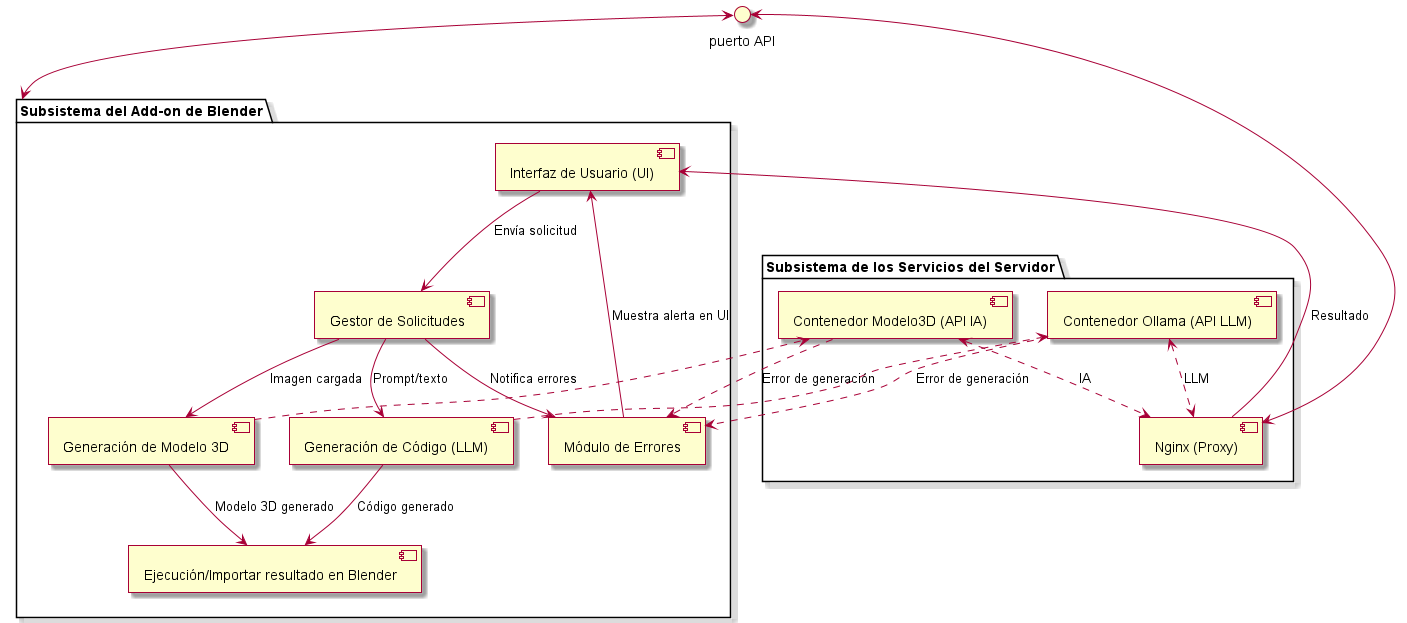
\includegraphics[width=1.1\textwidth]{figs/DiagramaArquitecturaGeneral.png}
  \caption{Diagrama de arquitectura general del sistema.}
  \label{fig:diagramaAGS}
\end{figure}

El primer subsistema consiste en el add-on de Blender, el cual proporciona la interfaz gráfica que el usuario/a emplea para interactuar al cargar imágenes, exportar los resultados de la generación 3D o utilizar modelos de inteligencia artificial. Este subsistema también gestiona las solicitudes tanto al modelo de lenguaje \gls{llm} como al modelo de generación de elementos 3D, procesa las respuestas de las \glspl{ia} generando el código Python en el caso del modelo \gls{llm} o generando el modelo 3D con el modelo generativo 3D y ejecuta dicho código Python o posiciona el modelo 3D en el entorno de Blender. Todo esto se realiza de manera no bloqueante para la aplicación, manejando cualquier posible error que ocurra e informando de ello.

El segundo subsistema está constituido por el servicio dockerizado, el cual alberga la API sobre Nginx que actúa como el componente orquestador principal y proxy, redirigiendo todas las solicitudes al modelo de \gls{ia} pertinente. En consecuencia, los demás componentes comprenden el contenedor del modelo de \gls{llm} y el contenedor del modelo generativo 3D, los cuales procesan las solicitudes recibidas y generan una respuesta o informan de un error.

% Imagen diagrama de arquitectura general del sistema


\section{Arquitectura de componentes}
% A partir de la especificación realizada en la sección \ref{sec:especificaciones-sistema} del Capítulo \ref{ch:requisitos} y la tecnología seleccionada en la sección \ref{sec:evaluacion-tecnologias} del Capítulo \ref{ch:estado-arte}, se debe construir el diagrama de componentes UML que represente la arquitectura de referencia del sistema. 
% En este diagrama se deben identificar los componentes principales del sistema y las relaciones entre ellos, pasando a detallar los subcomponentes de cada uno de ellos en secciones posteriores.
A continuación, se presentan los diagramas de componentes correspondientes a cada uno de los subsistemas del sistema propuesto, junto con sus respectivos diagramas de secuencia, los cuales describen en detalle las funciones específicas que ejecuta cada conjunto de componentes. Además, se indica el entorno tecnológico y el software utilizado en la implementación de dichas funcionalidades, permitiendo una visión clara de la distribución estructural y del flujo operativo dentro de la arquitectura del sistema. Es importante señalar que el elemento relacionado con la interfaz de usuario no se ha abordado en esta sección, porque en el apartado titulado "Wireframe de la pantalla del Add-on", se describe detalladamente esa interfaz junto con el correspondiente wireframe de la misma.

\subsection{Subsistema del add-on de Blender}
Este subsistema corresponde al complemento (add-on) desarrollado para su integración en el entorno Blender, permitiendo su instalación en múltiples dispositivos siempre que se utilice la versión 3.6 del software. En esta sección se analiza la estructura interna del complemento, describiendo el flujo completo de procesamiento, que abarca desde la entrada de una imagen o instrucción por parte del usuario hasta la recepción, ejecución, importación y exportación de resultados generados por los modelos de inteligencia artificial en el entorno de Blender. Este subsistema ha sido íntegramente desarrollado utilizando el lenguaje Python, dado que este es el lenguaje requerido para la elaboración de complementos en Blender.

La Figura~\ref{fig:diagramaGS1} presenta el diagrama de componentes del gestor de solicitudes del add-on. Este módulo actúa como núcleo de enrutamiento en el add-on, determinando si la petición debe ser redirigida al LLM o al modelo generativo 3D, gestionando dicha decisión mediante la invocación de la función Fetch correspondiente. Además, en caso de producirse errores durante el proceso, estos se comunican al módulo de notificación, que a su vez informa al usuario.
% Imagen diagrama componente 1
\begin{figure}[h!tp]
  \centering
  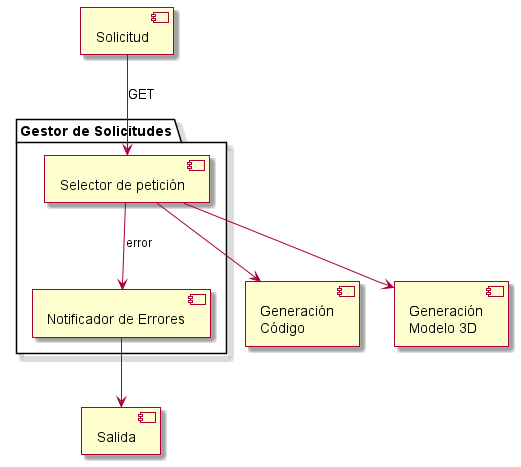
\includegraphics[width=0.8\textwidth]{figs/DiagramaComponentesGS.png}
  \caption{Diagrama de componentes del gestor de solicitudes del add-on.}
  \label{fig:diagramaGS1}
\end{figure}
El diagrama de secuencia asociado, mostrado en la Figura~\ref{fig:diagramaGS2}, detalla de manera precisa el comportamiento dinámico de este flujo.

% Imagen diagrama secuencia 1
\begin{figure}[h!tp]
  \centering
  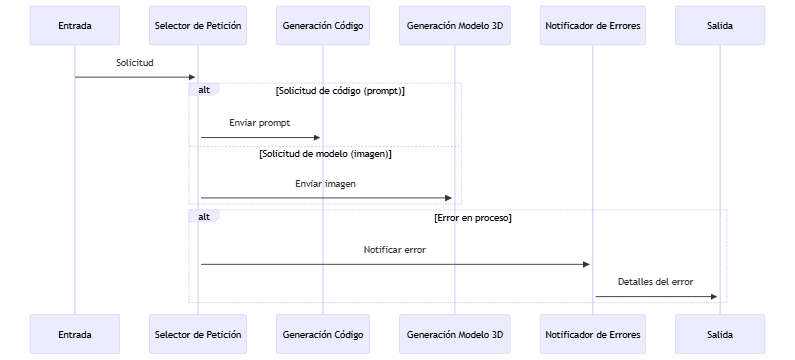
\includegraphics[width=1.1\textwidth]{figs/DiagramaSecuenciaGS.png}
  \caption{Diagrama de secuencia del gestor de solicitudes del add-on.}
  \label{fig:diagramaGS2}
\end{figure}



Por otro lado, la Figura~\ref{fig:diagramaGLLM1} presenta el diagrama de componentes correspondiente al módulo de generación de código Python, cuya función principal es gestionar el envío del prompt textual introducido por el usuario hacia el contenedor de Docker que aloja el modelo \gls{llm} de Ollama, a través de la API REST que integra el modelo de Ollama. La respuesta generada por el modelo es procesada mediante un filtro lógico, encargado de extraer exclusivamente el bloque de código Python relevante. Una vez depurado, el resultado se redirige al módulo de salida para su visualización o ejecución. En caso de que se produzcan errores durante la solicitud (fetch) o en el filtrado de la respuesta, estos son canalizados hacia el módulo de gestión de errores, el cual emite una notificación informativa hacia la salida correspondiente.
El comportamiento detallado de este proceso se encuentra descrito en el diagrama de secuencia de la Figura~\ref{fig:diagramaGLLM2}.
% Imagen diagrama componente 2
\begin{figure}[h!tp]
  \centering
  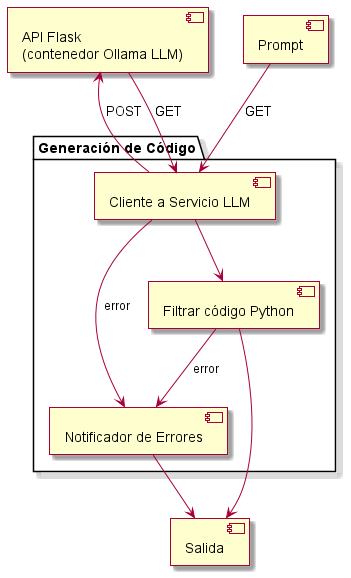
\includegraphics[width=0.5\textwidth]{figs/DiagramaComponentesGC.png}
  \caption{Diagrama de componentes de la generación de código.}
  \label{fig:diagramaGLLM1}
\end{figure}

% Imagen diagrama secuencia 2
\begin{figure}[h!tp]
  \centering
  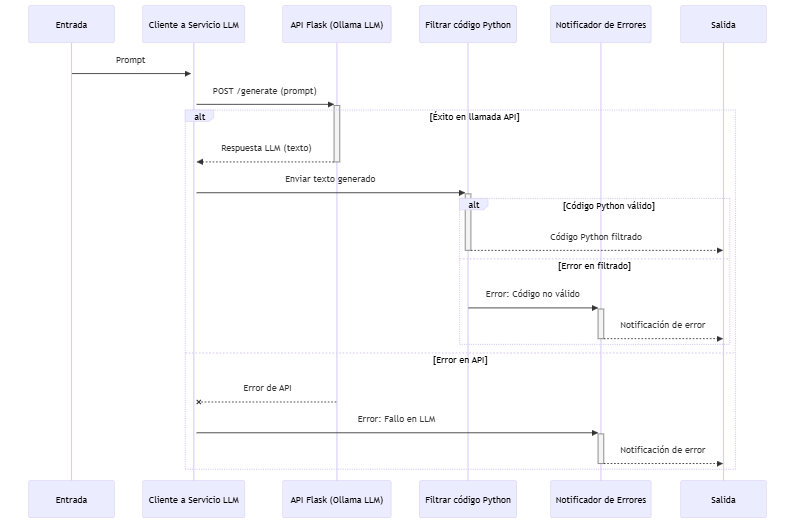
\includegraphics[width=1.1\textwidth]{figs/DiagramaSecuenciaGC.png}
  \caption{Diagrama de secuencia de la generación de código.}
  \label{fig:diagramaGLLM2}
\end{figure}

La Figura~\ref{fig:diagramaGM3D1} representa el diagrama de componentes correspondiente al proceso de generación de modelos tridimensionales a partir de imágenes. Este módulo es responsable de recibir una imagen proporcionada por el usuario y transmitirla, mediante una solicitud fetch, al contenedor Docker donde se ejecuta el modelo de inteligencia artificial 3D, accesible a través de la API Flask propia del modelo. Una vez procesada la imagen, el sistema retorna un modelo 3D generado, que es dirigido directamente al módulo de salida para su posterior utilización. En caso de producirse errores durante el envío de la solicitud o en la gestión de la respuesta, dichos errores son derivados al gestor de notificaciones, encargado de informar al usuario mediante la salida correspondiente.
% Imagen diagrama componente 3
\begin{figure}[h!tp]
  \centering
  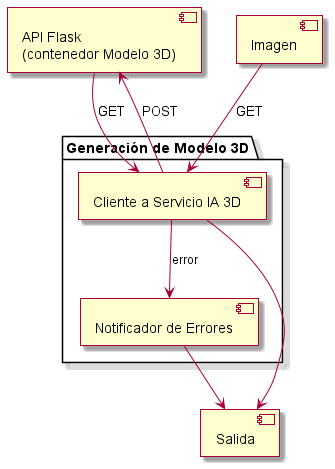
\includegraphics[width=0.5\textwidth]{figs/DiagramaComponentesGM3D.png}
  \caption{Diagrama de componentes de la generación del modelo 3D.}
  \label{fig:diagramaGM3D1}
\end{figure}
El flujo detallado de esta operación se encuentra descrito en el diagrama de secuencia de la Figura~\ref{fig:diagramaGM3D2}.
% Imagen diagrama secuencia 3
\begin{figure}[h!tp]
  \centering
  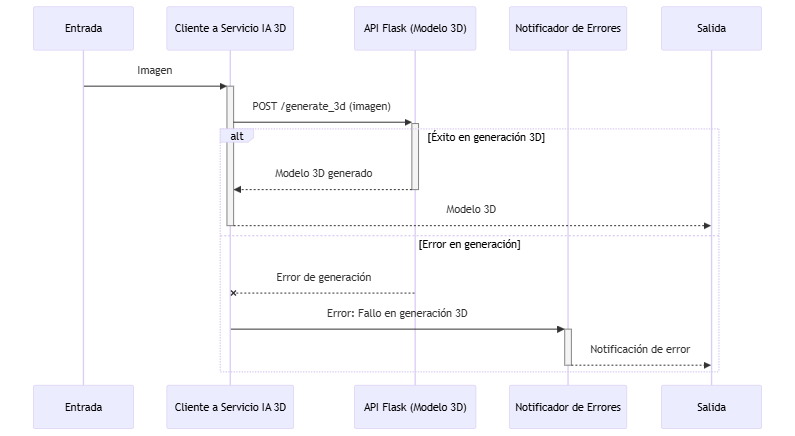
\includegraphics[width=1.1\textwidth]{figs/DiagramaSecuenciaGM3D.png}
  \caption{Diagrama de secuencia de la generación del modelo 3D.}
  \label{fig:diagramaGM3D2}
\end{figure}

La Figura~\ref{fig:diagramaEIB1} presenta el diagrama de componentes del módulo responsable de las operaciones de ejecución, importación y exportación dentro del entorno de Blender.
% Imagen diagrama componente 4
\begin{figure}[h!tp]
  \centering
  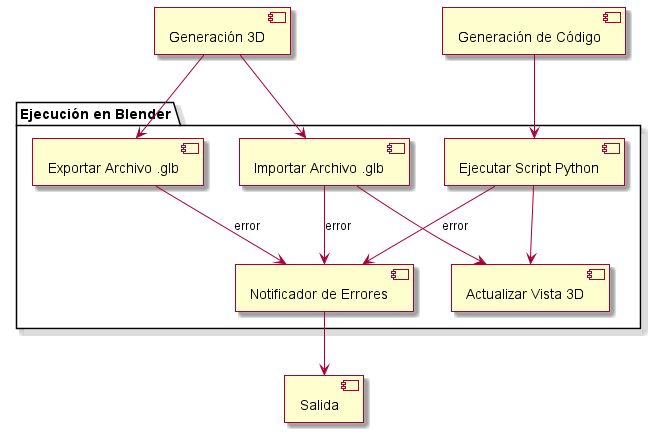
\includegraphics[width=0.8\textwidth]{figs/DiagramaComponentesEIB.png}
  \caption{Diagrama de componentes de la ejecución/importación/exportación en Blender.}
  \label{fig:diagramaEIB1}
\end{figure}
Este componente actúa en función del tipo de entrada recibida, si se trata de código Python, el sistema procede a ejecutarlo directamente sobre la escena activa, actualizando posteriormente la vista 3D para reflejar los cambios. En caso de recibir un modelo 3D generado, el sistema lo importa automáticamente en la escena, habilitando además su exportación en formato .glb, y actualiza de igual manera la visualización en tiempo real. Ante cualquier fallo detectado durante la ejecución del script, la importación del modelo o el proceso de exportación, el error es redirigido al gestor de errores, que se encarga de emitir una notificación al usuario a través del canal de salida.
El comportamiento detallado de este subsistema puede consultarse en el diagrama de secuencia de la Figura~\ref{fig:diagramaEIB2}.
% Imagen diagrama secuencia 4
\begin{figure}[h!tp]
  \centering
  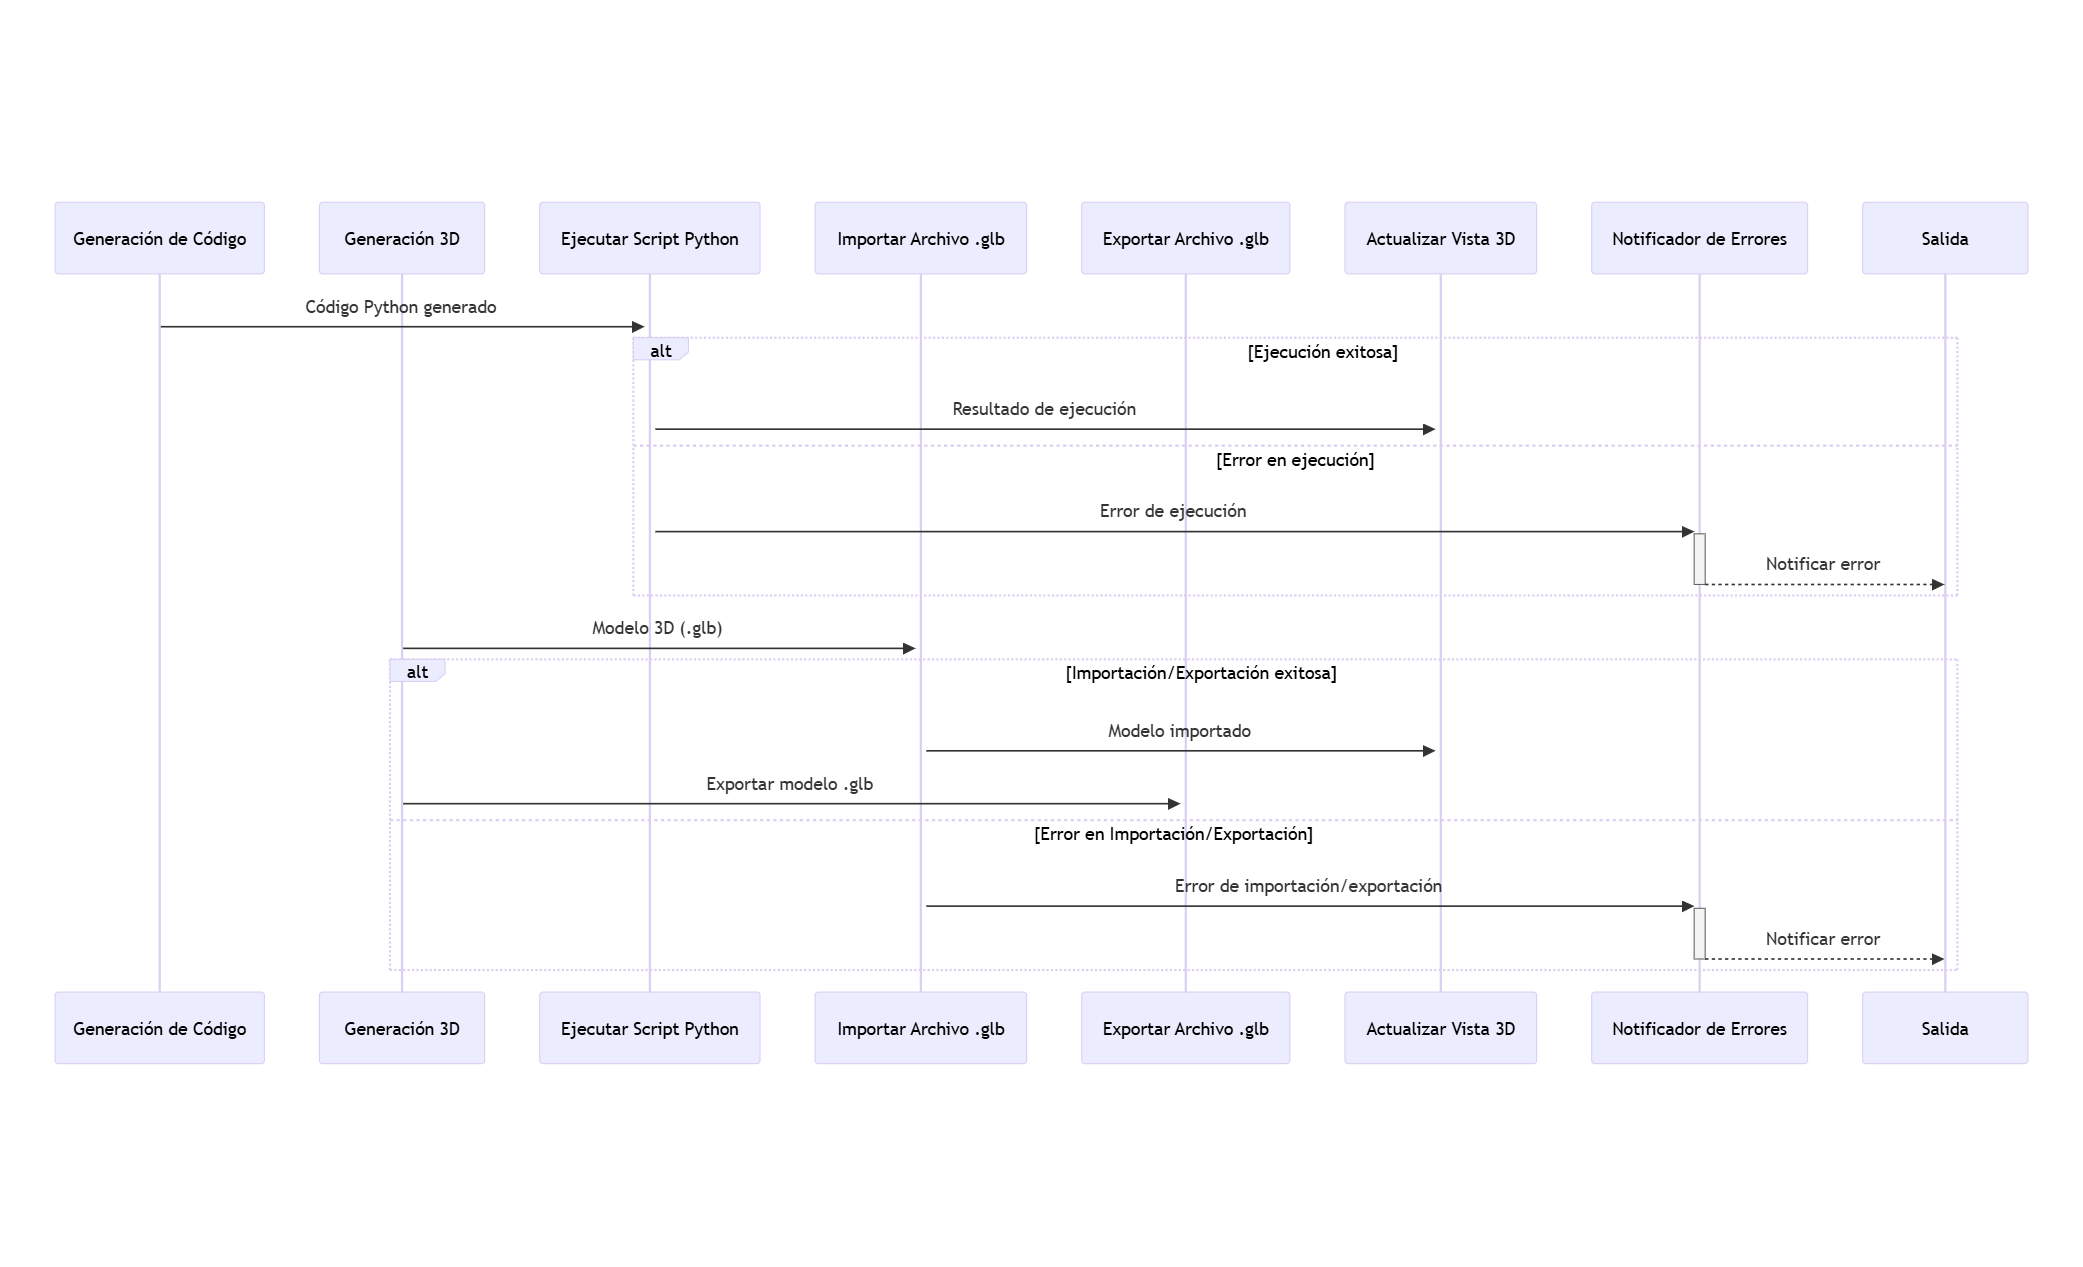
\includegraphics[width=1.1\textwidth]{figs/DiagramaSecuenciaEIB.png}
  \caption{Diagrama de secuencia de la ejecución/importación/exportación en Blender.}
  \label{fig:diagramaEIB2}
\end{figure}



Finalmente, como elemento final del subsistema del add-on de Blender, se presenta la Figura~\ref{fig:diagramaME1}, que ilustra el diagrama de componentes del módulo de gestión de errores. Este módulo tiene como principal función la captura, el procesamiento y el formateo de cualquier tipo de error procedente de otros subsistemas y del mismo. Una vez formateado, el mensaje de error es transmitido al componente de interfaz de usuario mediante la salida adecuada, lo que permite su visualización de manera clara para el usuario. El comportamiento de este módulo, así como su interacción con el resto del sistema, están detallados en el diagrama de secuencia de la Figura~\ref{fig:diagramaME2}.
% Imagen diagrama componente 5
\begin{figure}[h!tp]
  \centering
  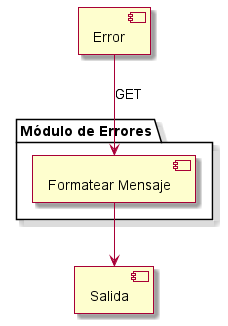
\includegraphics[width=0.4\textwidth]{figs/DiagramaComponentesME.png}
  \caption{Diagrama de componentes del módulo de errores.}
  \label{fig:diagramaME1}
\end{figure}

% Imagen diagrama secuencia 5
\begin{figure}[h!tp]
  \centering
  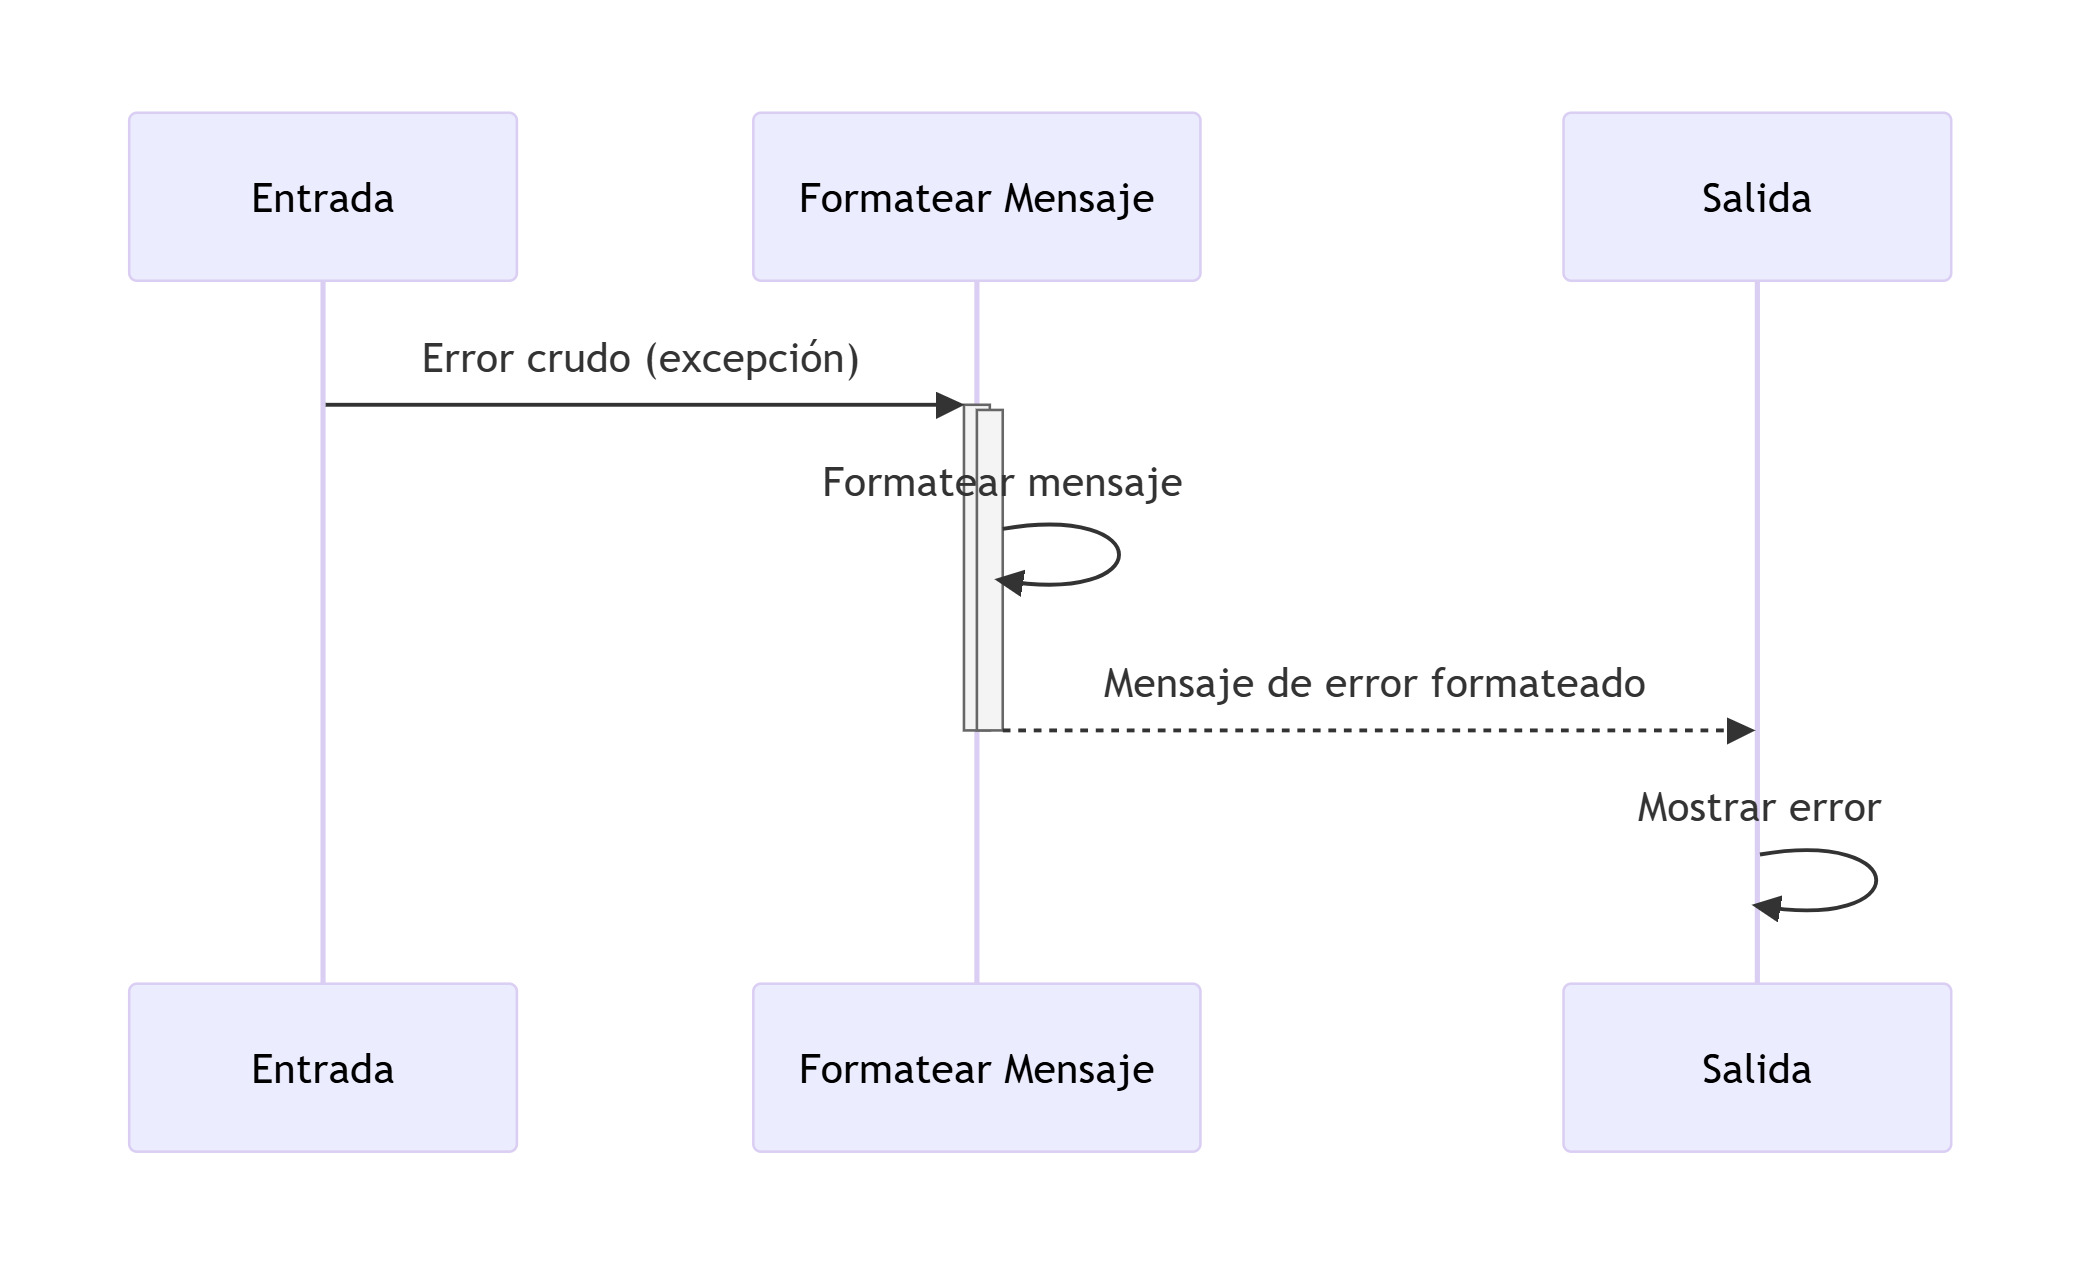
\includegraphics[width=0.8\textwidth]{figs/DiagramaSecuenciaME.png}
  \caption{Diagrama de secuencia del módulo de errores.}
  \label{fig:diagramaME2}
\end{figure}


\subsection{Subsistema de los servicios del servidor}
El segundo y último subsistema corresponde a la infraestructura de servicios dockerizados, diseñada para hacer de proxy y orquestar dinámicamente las solicitudes dirigidas a los modelos de inteligencia artificial, tanto al modelo de lenguaje \gls{llm} como al modelo generativo 3D, a través de una API REST desarrollada con Nginx. Este enfoque de implementación ofrece una arquitectura flexible y escalable, idónea para su posible integración en entornos de producción o sistemas empresariales, al permitir la ejecución concurrente de múltiples peticiones sin bloquear el flujo de procesamiento, gracias a la naturaleza asincrónica del sistema. En esta sección se detalla la estructura interna del servidor de \gls{ia}, describiendo el flujo de procesamiento desde la recepción de entradas en formato texto o imagen a través de la API/proxy, hasta su encaminamiento hacia el contenedor correspondiente que aloja el modelo adecuado. Una vez procesadas, las respuestas generadas por los modelos son gestionadas y devueltas al complemento de Blender, garantizando una integración eficiente entre cliente y servidor. Este subsistema ha sido implementado utilizando el proxy mediante el archivo de configuración de Nginx, mientras que la definición de contenedores y su configuración se ha realizado mediante los lenguajes Dockerfile DSL y YAML para los archivos de Docker Compose del despliegue local.

La Figura~\ref{fig:diagramaAPI1} muestra el diagrama de componentes correspondiente al módulo de la API que hace de proxy mediante Nginx, que actúa como punto central de enrutamiento y coordinación dentro del servidor de inteligencia artificial.

% Imagen diagrama componente 6
\begin{figure}[h!tp]
  \centering
  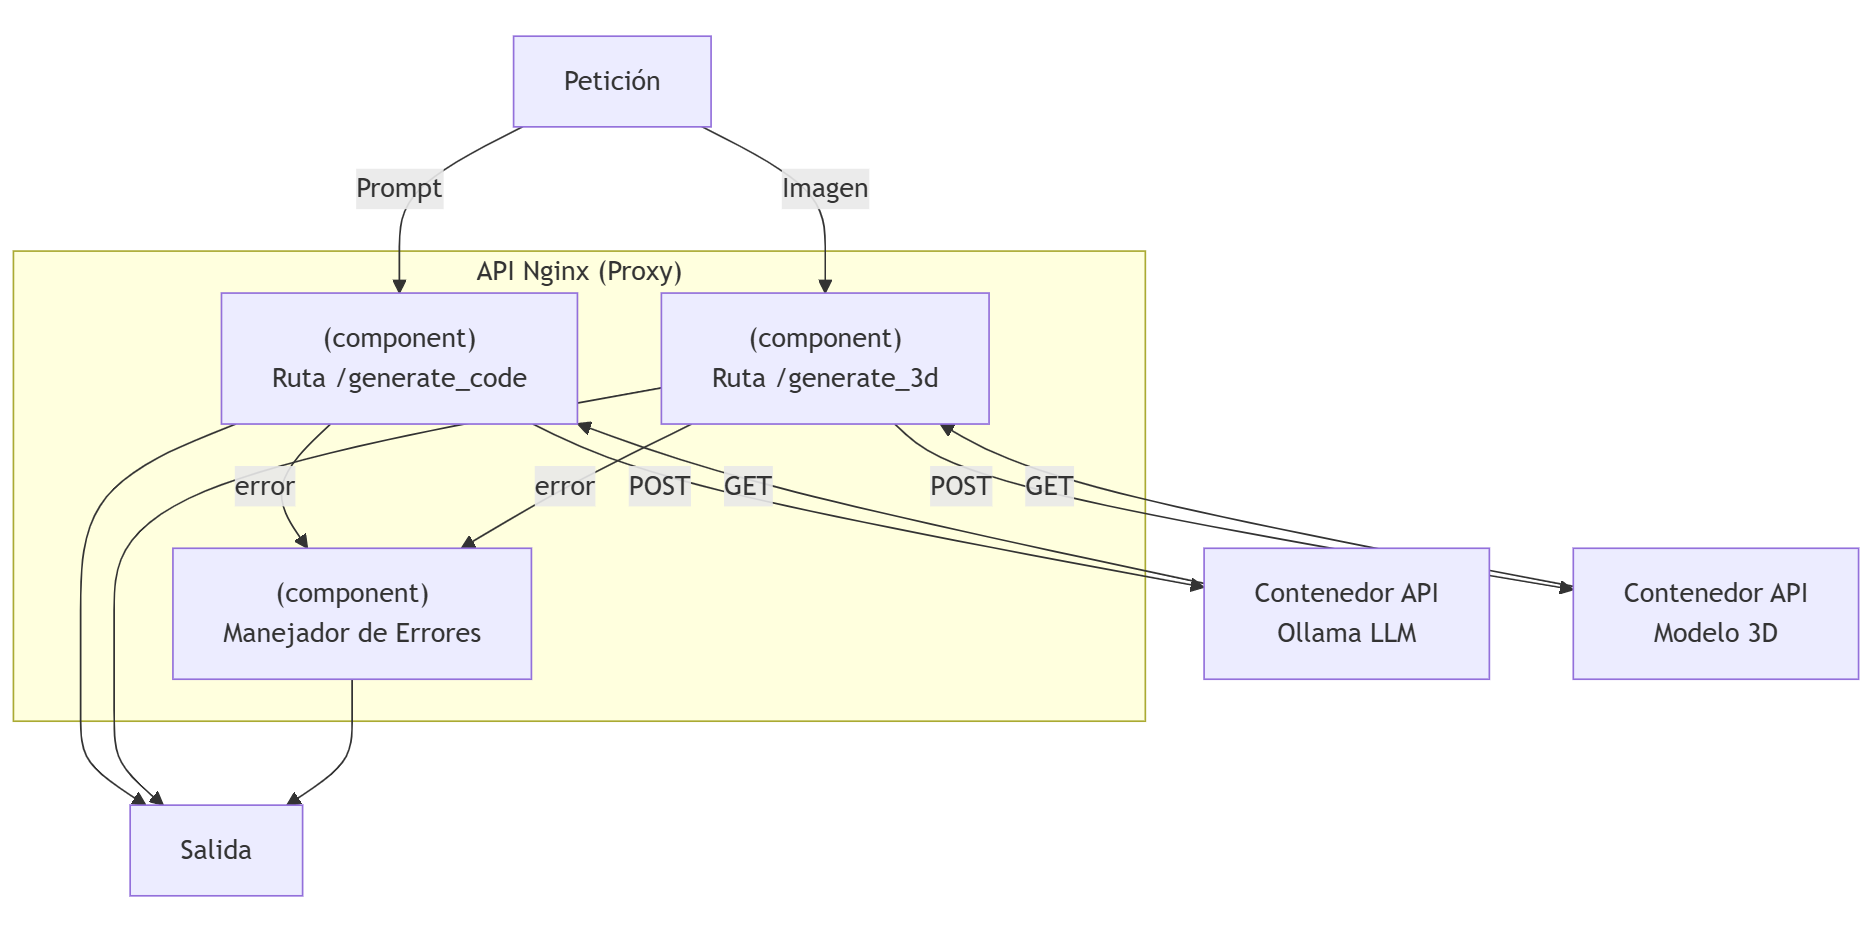
\includegraphics[width=1.1\textwidth]{figs/DiagramaComponentesAPI.png}
  \caption{Diagrama de componentes de la API Nginx.}
  \label{fig:diagramaAPI1}
\end{figure}

Este componente es responsable de analizar cada solicitud entrante proveniente del add-on, identificando si se trata de un prompt textual o de una imagen, y en función de ello, redirigirla al contenedor apropiado, el que aloja el modelo LLM de Ollama o el correspondiente al modelo generativo 3D. La API se encarga de invocar el contenedor seleccionado, gestionar la ejecución del modelo y recoger la respuesta generada, la cual es posteriormente enviada de vuelta al add-on a través del canal de salida del componente. En caso de que se produzcan errores durante el procesamiento, ya sea en la fase de redirección, ejecución o respuesta, estos son transmitidos al módulo de notificación, que se encarga de retornar un mensaje de error informativo al add-on. El diagrama de secuencia presentado en la Figura~\ref{fig:diagramaAPI2} ilustra de manera exhaustiva el flujo de operaciones y decisiones que configuran este comportamiento.


% Imagen diagrama secuencia 6
\begin{figure}[h!tp]
  \centering
  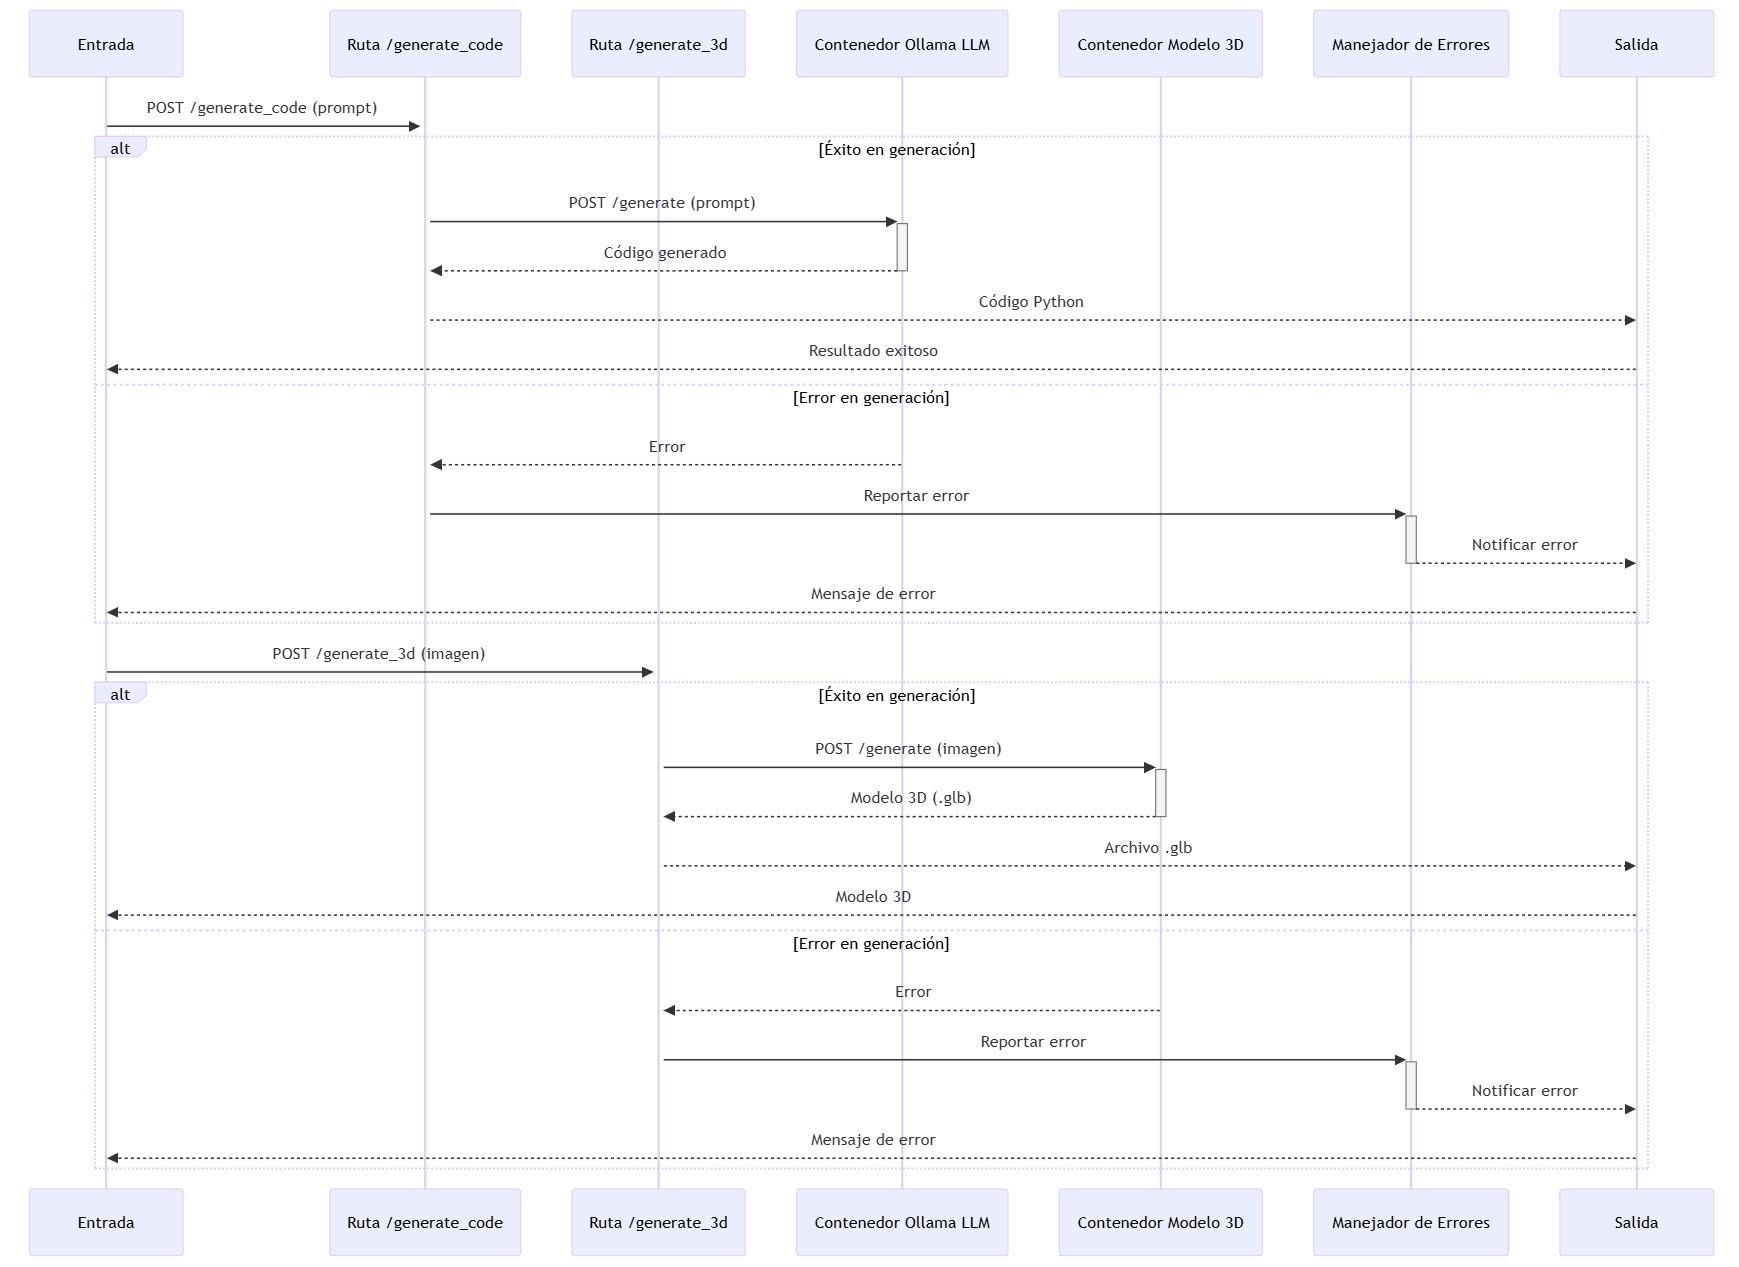
\includegraphics[width=1.1\textwidth]{figs/DiagramaSecuenciaAPI.png}
  \caption{Diagrama de secuencia de la API Nginx.}
  \label{fig:diagramaAPI2}
\end{figure}



La Figura~\ref{fig:diagramaMLLM1} representa el diagrama de componentes del contenedor que aloja el modelo LLM provisto por Ollama, concretamente utilizando la imagen correspondiente al modelo Dolphin-Mistral.
% Imagen diagrama componente 7
\begin{figure}[h!tp]
  \centering
  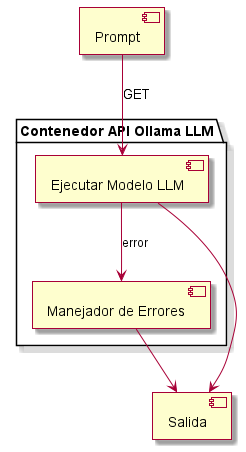
\includegraphics[width=0.4\textwidth]{figs/DiagramaComponentesMLLM.png}
  \caption{Diagrama de componentes del contenedor del modelo LLM.}
  \label{fig:diagramaMLLM1}
\end{figure}
Este componente es responsable de recibir los prompts textuales enviados por el proxy Nginx, obtenerlas mediante la API REST propia de Ollama, ejecutar el modelo LLM sobre dicha entrada, y generar como resultado una respuesta estructurada que incluye el código Python solicitado. Una vez completado el proceso de inferencia, la salida es reenviada a la API y el proxy para su posterior transmisión al add-on. En caso de producirse errores durante la ejecución del modelo, estos son capturados y redirigidos al módulo de notificación de errores, el cual se encarga de generar una respuesta adecuada que será igualmente retornada a través del proxy. El comportamiento detallado de este flujo, así como las interacciones entre componentes, se especifica en el diagrama de secuencia mostrado en la Figura~\ref{fig:diagramaMLLM2}.


% Imagen diagrama secuencia 7
\begin{figure}[h!tp]
  \centering
  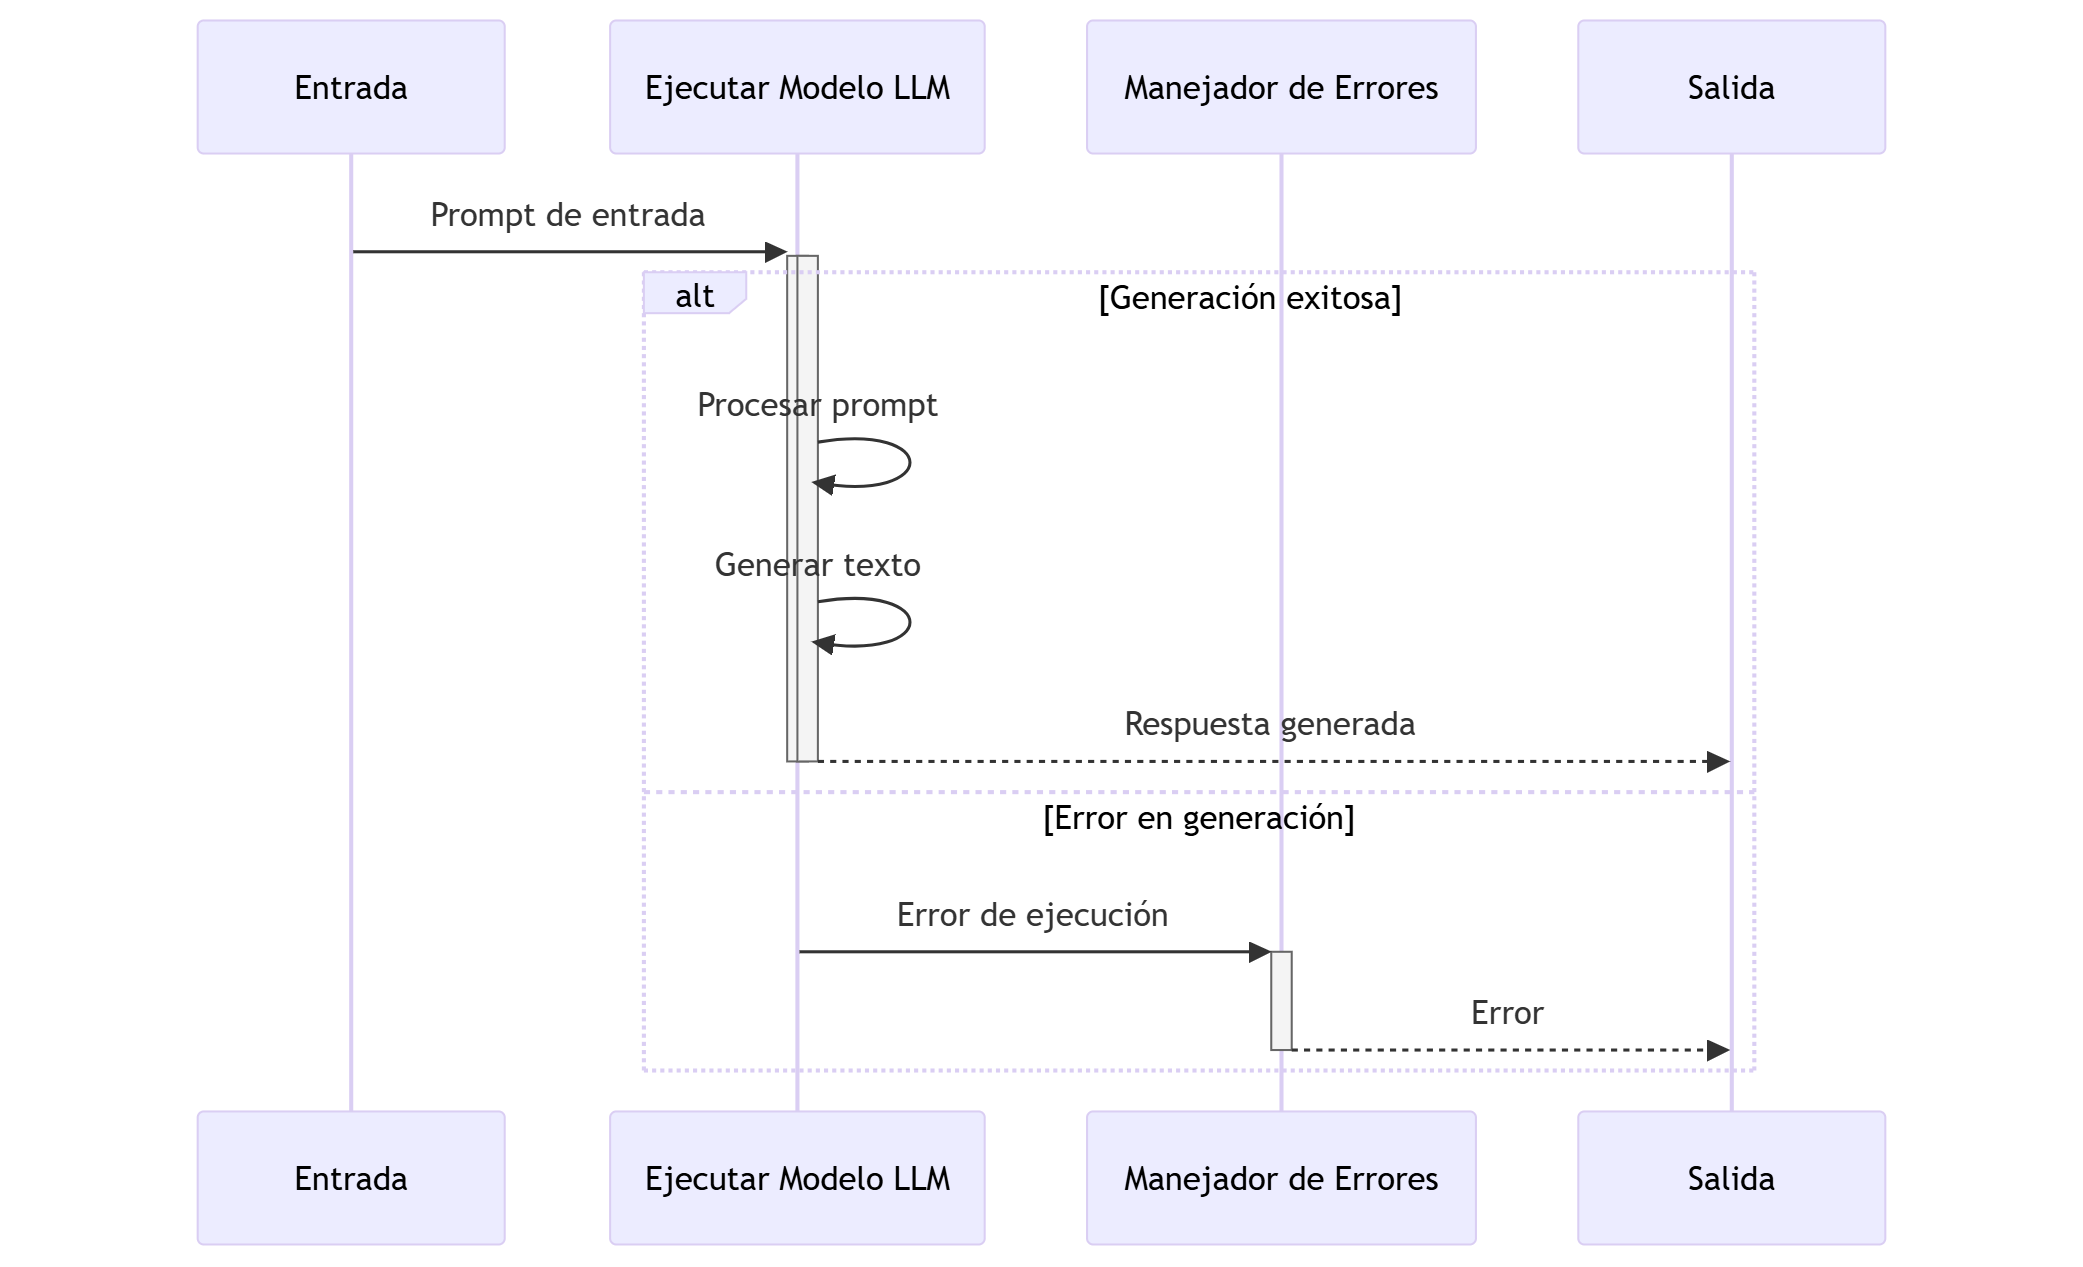
\includegraphics[width=1.0\textwidth]{figs/DiagramaSecuenciaMLLM.png}
  \caption{Diagrama de secuencia del contenedor del modelo LLM.}
  \label{fig:diagramaMLLM2}
\end{figure}



Como último componente del subsistema de infraestructura de servicios dockerizados y al mismo tiempo como subsistema final del proyecto, se presenta en la Figura~\ref{fig:diagramaMIA3D1} el diagrama de componentes correspondiente al contenedor del modelo de generación 3D mediante \gls{ia}. Este módulo está diseñado para recibir, a través del proxy Nginx, una imagen proporcionada por el add-on y procesarla mediante la API Flask custom del contenedor y utilizando una instancia personalizada del modelo TripoSR, especializado en reconstrucción tridimensional a partir de imágenes. Tras la ejecución del modelo, se genera una respuesta estructurada que contiene el modelo 3D del objeto presente en la imagen de entrada, el cual es enviado nuevamente a la API del contenedor y finalmente al proxy general para su posterior entrega al add-on de Blender. En caso de que se produzcan errores durante la ejecución del modelo TripoSR, estos son capturados por el sistema y gestionados por el módulo de notificación de errores, que transmite el mensaje correspondiente de vuelta a través del canal de salida. El funcionamiento detallado de este flujo se encuentra descrito en el diagrama de secuencia de la Figura~\ref{fig:diagramaMIA3D2}. Es importante señalar que tanto la API Flask como la imagen Docker de este contenedor de Docker y modelo de inteligencia artificial han sido desarrolladas de forma personalizada. Para ello, se ha empleado el lenguaje Python en la implementación de la API, así como un lenguaje específico de dominio (DSL) en la elaboración de los archivos de configuración de Docker.
% Imagen diagrama componente 8
\begin{figure}[h!tp]
  \centering
  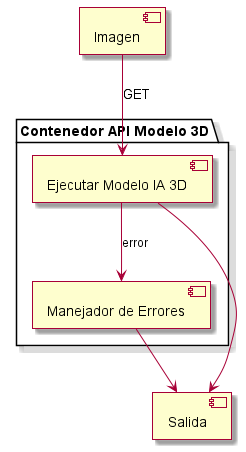
\includegraphics[width=0.4\textwidth]{figs/DiagramaComponentesMIA3D.png}
  \caption{Diagrama de componentes del contenedor del modelo IA 3D.}
  \label{fig:diagramaMIA3D1}
\end{figure}

% Imagen diagrama secuencia 8
\begin{figure}[h!tp]
  \centering
  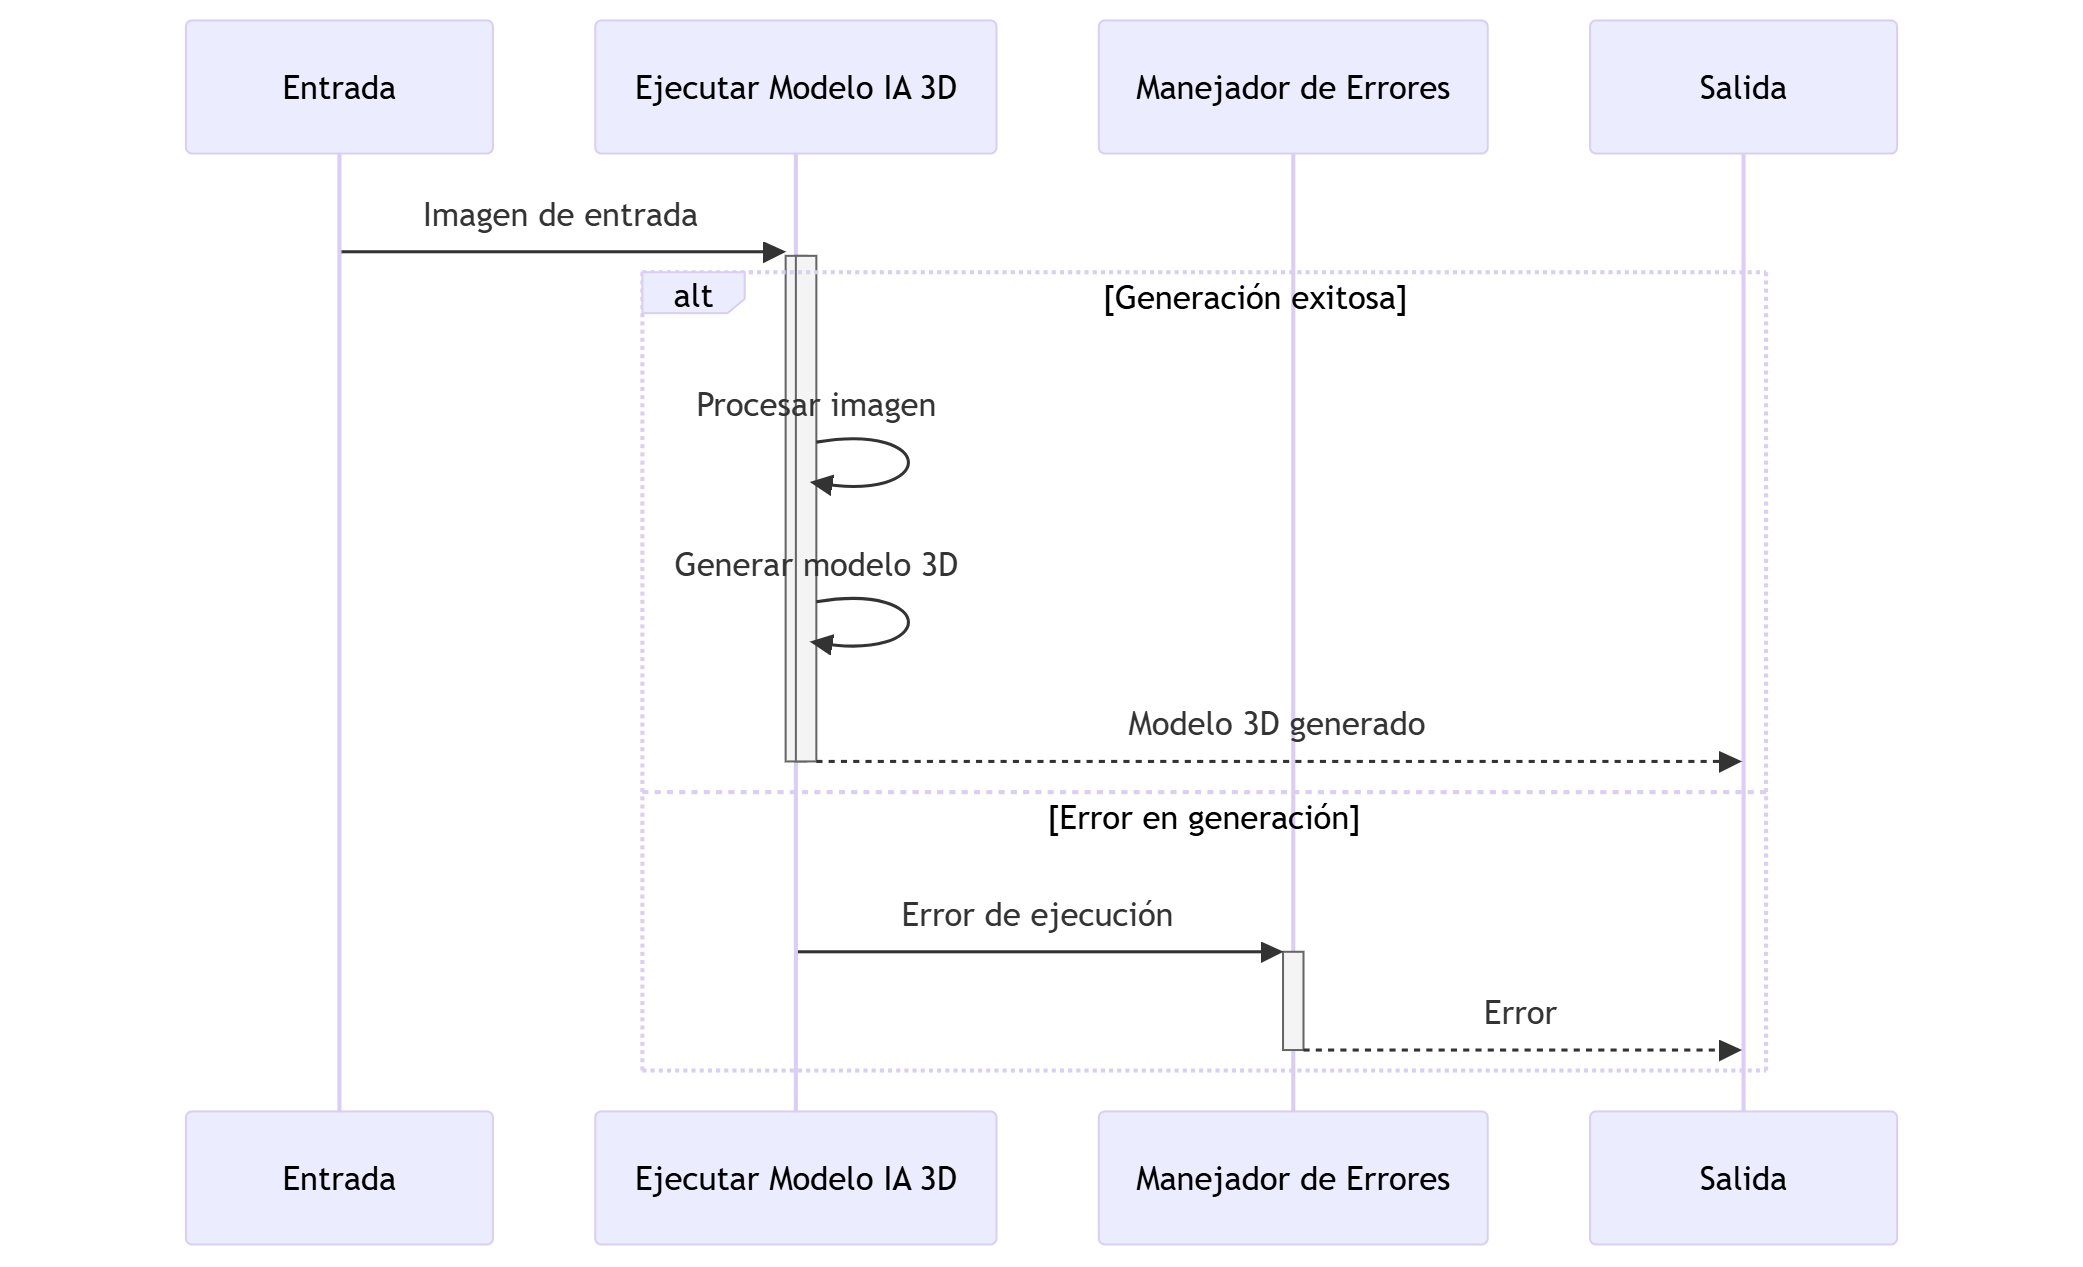
\includegraphics[width=1.0\textwidth]{figs/DiagramaSecuenciaMIA3D.png}
  \caption{Diagrama de secuencia del contenedor del modelo IA 3D.}
  \label{fig:diagramaMIA3D2}
\end{figure}



\section{Despliegue del sistema}
% En esta sección se debe presentar el diagrama de despliegue del sistema, que muestre la arquitectura física del sistema y cómo se distribuyen los componentes en los nodos físicos o virtuales que lo componen.
% En otras palabras, para cada componente principal del sistema se identifica en que servidor físico o virtual se va a ejecutar.

% Se puede definir un despligue de desarrollo (el despliegue que se tiene en el portátil mientras se trabaja), uno de producción (despliegue final o real) y uno de pruebas (lo más parecido posible al real).

En esta sección se expone la implementación y el despliegue completo del sistema, con especial énfasis en la configuración basada en Docker Compose, utilizada durante la fase de pruebas y validación funcional. La Figura~\ref{fig:diagramaDGS} muestra una visión general de la arquitectura de despliegue adoptada, diferenciando claramente los dos dispositivos clave involucrados en la operación del sistema.

% Imagen diagrama de despliegue general del sistema
\begin{figure}[h!tp]
  \centering
  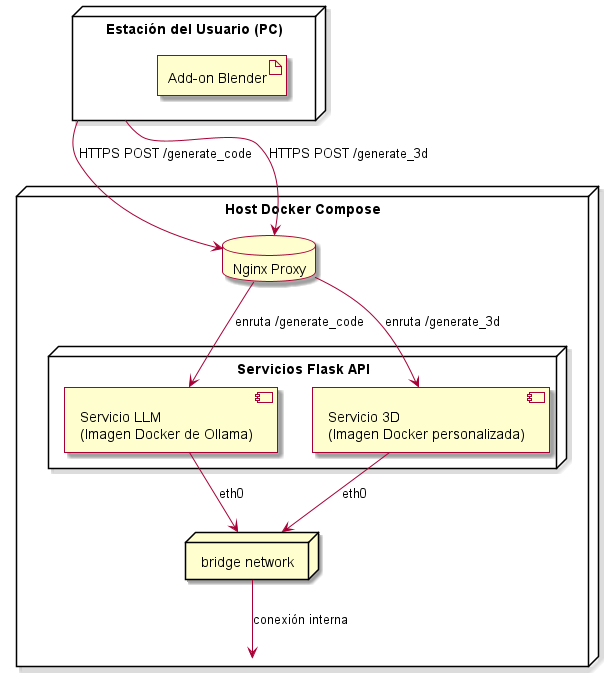
\includegraphics[width=0.8\textwidth]{figs/DiagramaDespliegueGeneral.png}
  \caption{Diagrama de despliegue general del sistema.}
  \label{fig:diagramaDGS}
\end{figure}

Por un lado, se encuentra el dispositivo local del usuario/a, en el que se instala el add-on para Blender, el cual actúa como interfaz principal y punto de interacción con los modelos de inteligencia artificial. Por otro lado, se encuentra la infraestructura en la nube (cloud), simulada en este proyecto mediante un entorno de contenedores Docker. Esta capa es responsable de la ejecución de los modelos de IA a través de un proxy Nginx que intermedia entre los distintos contenedores y las API de cada servicio.

La comunicación entre ambos componentes se realiza mediante un proxy de Nginx y las API REST de los modelos, que permite el envío de solicitudes HTTPS al servicio de Nginx y finalmente a la API del servicio alojada en Flask. Dado que todo el entorno se ejecuta en una única máquina física durante el desarrollo y las pruebas, todas las peticiones se dirigen a \verb|localhost| (127.0.0.1).

Una descripción más detallada del entorno de contenedores se presenta en la Figura~\ref{fig:diagramaDDC},
% Imagen diagrama de despliegue de Docker Compose
\begin{figure}[h!tp]
  \centering
  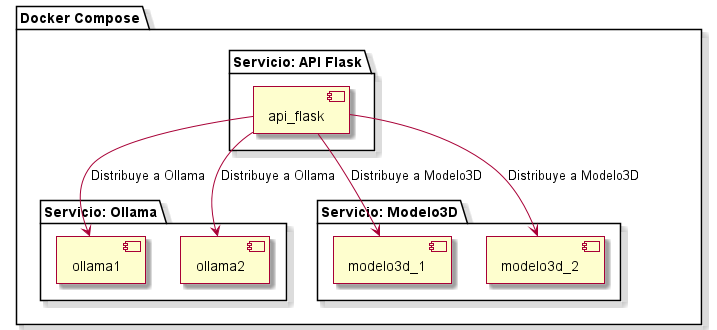
\includegraphics[width=0.8\textwidth]{figs/DiagramaDespliegueDockerCompose.png}
  \caption{Diagrama de despliegue local.}
  \label{fig:diagramaDDC}
\end{figure}
donde se observa que el nodo cloud, ejecutado sobre Docker, está compuesto por tres subcomponentes principales:

\begin{enumerate}
  \item \textbf{Contenedor de la API Nginx}: este módulo actúa como intermediario, recibiendo las solicitudes del add-on y redirigiéndolas al API REST del servicio correspondiente en función del tipo de petición recibida.
  \item \textbf{Contenedor de la API}: este módulo existe en cada contenedor de un modelo de IA recibe las solicitudes del proxy y las ejecuta en su modelo de IA correspondiente.
  \item \textbf{Servicio de modelos LLM (Ollama)}: encargado de procesar los prompts enviados por el usuario/a para generar código en Python. Este servicio se despliega con múltiples modelos LLM de forma concurrente, permitiendo la gestión simultánea de varias peticiones.
  \item \textbf{Servicio de modelado 3D}: responsable de la conversión de imágenes en objetos tridimensionales mediante modelos generativos 3D. Al igual que el anterior, este componente también admite múltiples instancias del modelo, lo que garantiza la capacidad de respuesta ante múltiples solicitudes concurrentes.
\end{enumerate}

Esta arquitectura modular basada en contenedores permite escalar los distintos servicios de manera independiente, además de facilitar el mantenimiento, la portabilidad y el despliegue del sistema en entornos distribuidos. La Figura \ref{fig:esbozoDespliegue} ilustra el esquema preliminar del despliegue en producción previsto para este sistema, que en esta ocasión se llevará a cabo localmente.

% Imagen esbozo
\begin{figure}[h!tp]
  \centering
  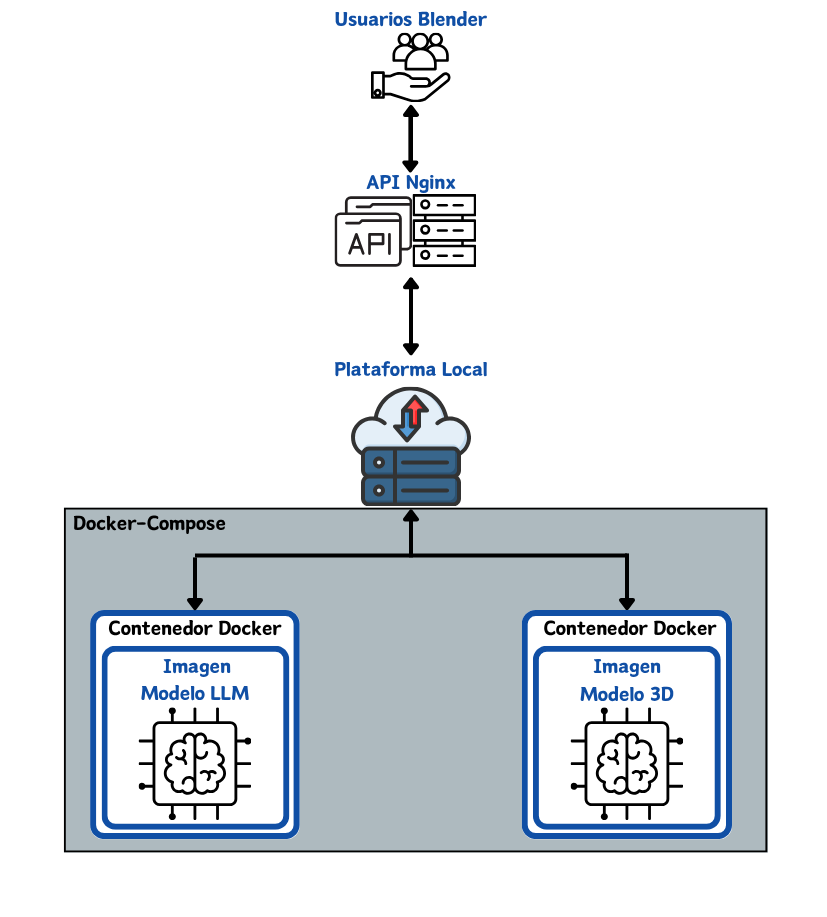
\includegraphics[width=0.8\textwidth]{figs/esbozoDespliegue.png}
  \caption{Esbozo del despliegue en producción del sistema.}
  \label{fig:esbozoDespliegue}
\end{figure}







\section{Wireframe de la pantalla del Add-on}

En esta sección, se presenta la Figura~\ref{fig:wireframeUI}, la cual ilustra el diseño del wireframe de la interfaz de usuario/a creada para el complemento de Blender denominado GenerativeCHAT, el cual ha sido diseñado para facilitar la interacción entre el usuario/a y los modelos de inteligencia artificial generativa integrados en el sistema. La interfaz se estructura en dos bloques funcionales principales: el Agente \gls{llm} y el Agente 3D, cada uno orientado a una tarea específica del flujo de trabajo.

En la parte superior se encuentra el Agente \gls{llm}, encargado de la generación automática de código Python adaptado al entorno de Blender. El usuario/a introduce una instrucción en lenguaje natural en el campo de entrada, y al activar la opción \emph{Generar código}, dicha instrucción es procesada por el modelo \gls{llm}. La respuesta es generada en forma de flujo continuo, lo que permite observar el proceso de respuesta de la \gls{ia}. Esta respuesta es representada en un campo de texto intermedio y en la pestaña de programación de Blender, también puede ser ejecutado el código resultante directamente dentro de Blender mediante el botón \emph{Ejecutar código}. Este mecanismo facilita una integración fluida entre el lenguaje natural y la automatización de tareas.

En la parte inferior, el Agente 3D permite al usuario/a generar modelos tridimensionales a partir de imágenes. A través del botón \emph{Cargar imagen}, se envía una imagen al modelo generativo 3D, el cual produce una reconstrucción volumétrica del contenido visual. Posteriormente, el modelo generado puede ser importado al entorno de Blender mediante la opción \emph{Cargar modelo} o exportado mediante \emph{Descargar modelo}.

% Imagen wireframe del diseño del add-on
\begin{figure}[h!tp]
  \centering
  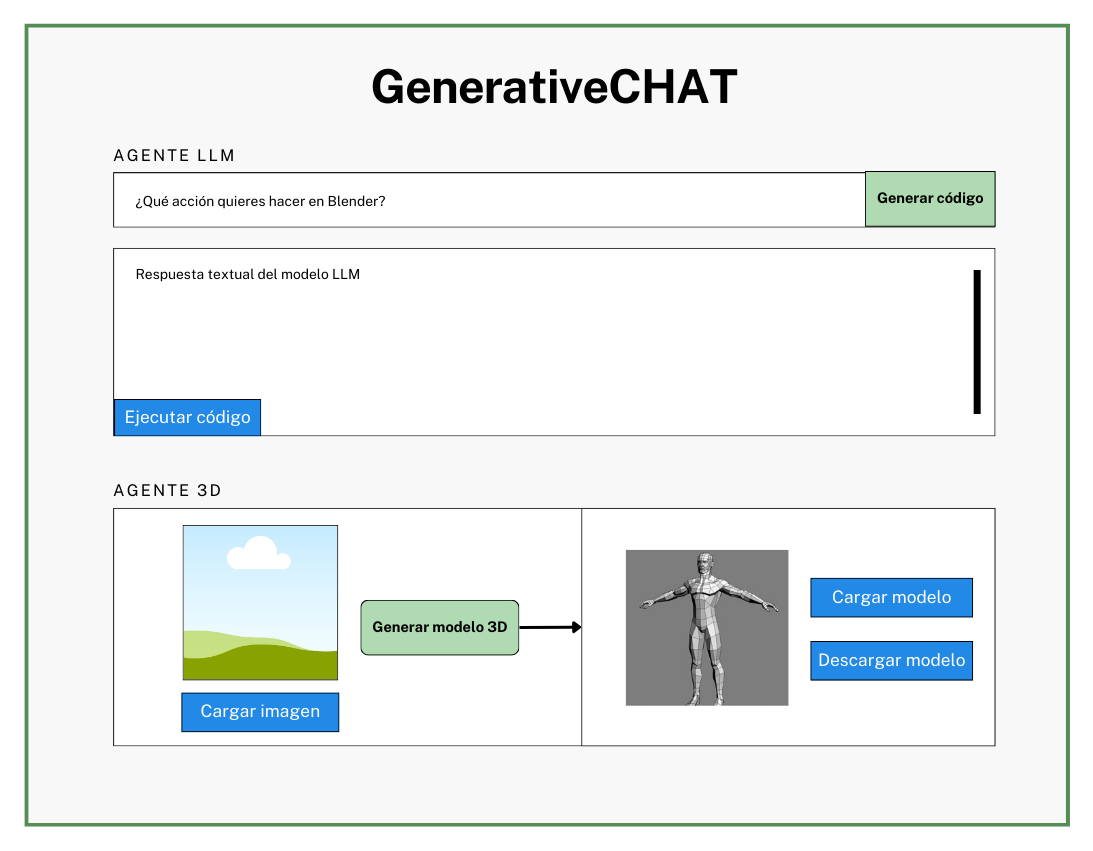
\includegraphics[width=0.8\textwidth]{figs/wireframeAddon.png}
  \caption{Wireframe del diseño del add-on.}
  \label{fig:wireframeUI}
\end{figure}

% En este caso se puede especificar el diagrama de clases final del diseño atendiendo al lenguaje de programación y a la tecnología seleccionada.
% Además será necesario, como mínimo, especificar el modelo físico de datos, en el lenguaje SQL propio de la base de datos relacional seleccionada, o el modelo de documentos, si se utiliza una base de datos NoSQL. 
